\documentclass[12pt,a4paper,titlepage,headinclude,bibtotoc]{scrartcl}

%---- Allgemeine Layout Einstellungen ------------------------------------------

% Für Kopf und Fußzeilen, siehe auch KOMA-Skript Doku
\usepackage[komastyle]{scrpage2}
\pagestyle{plain}
\setheadsepline{0.5pt}[\color{black}]
\automark[section]{chapter}


%Einstellungen für Figuren- und Tabellenbeschriftungen
\setkomafont{captionlabel}{\sffamily\bfseries}
\setcapindent{0em}


%---- Weitere Pakete -----------------------------------------------------------
% Die Pakete sind alle in der TeX Live Distribution enthalten. Wichtige Adressen
% www.ctan.org, www.dante.de

% Sprachunterstützung
\usepackage[ngerman]{babel}

% Benutzung von Umlauten direkt im Text
% entweder "latin1" oder "utf8"
\usepackage[utf8]{inputenc}

% Pakete mit Mathesymbolen und zur Beseitigung von Schwächen der Mathe-Umgebung
\usepackage{latexsym,exscale,stmaryrd,amssymb,amsmath}


\usepackage[nointegrals]{wasysym}
\usepackage{eurosym}

% Anderes Literaturverzeichnisformat
%\usepackage[square,sort&compress]{natbib}
\usepackage{hyperref}
% Für Farbe
\usepackage{color}
\usepackage{graphicx}
\usepackage{wrapfig}
\usepackage{subfigure}

% Caption neben Abbildung
\usepackage{sidecap}


% Befehl für "Entspricht"-Zeichen
\newcommand{\corresponds}{\ensuremath{\mathrel{\widehat{=}}}}
% Befehl für Errorfunction
\newcommand{\erf}[1]{\text{ erf}\ensuremath{\left( #1 \right)}}


%Fußnoten zwingend auf diese Seite setzen
\interfootnotelinepenalty=1000

%Für chemische Formeln (von www.dante.de)
%% Anpassung an LaTeX(2e) von Bernd Raichle
\makeatletter
\DeclareRobustCommand{\chemical}[1]{%
  {\(\m@th
   \edef\resetfontdimens{\noexpand\)%
       \fontdimen16\textfont2=\the\fontdimen16\textfont2
       \fontdimen17\textfont2=\the\fontdimen17\textfont2\relax}%
   \fontdimen16\textfont2=2.7pt \fontdimen17\textfont2=2.7pt
   \mathrm{#1}%
   \resetfontdimens}}
\makeatother
\usepackage{textcomp}
\usepackage{upgreek}
%\begin{document}
%$\upmu$
%\end{document}
%Honecker-Kasten mit $$\shadowbox{$xxxx$}$$
\usepackage{fancybox}

%SI-Package
\usepackage{siunitx}

%keine Einrückung, wenn Latex doppelte Leerzeile
\parindent0pt

%Bibliography \bibliography{literatur} und \cite{gerthsen}
%\usepackage{cite}
\usepackage{babelbib}
\selectbiblanguage{ngerman}

\usepackage{siunitx}
%\begin{document}
 % \SI{1.55}{\micro\metre}
\sisetup{math-micro=\text{µ},text-micro=µ}
\usepackage{amsmath}

\usepackage[verbose]{placeins}
%für \FloatBarrier

\begin{document}

\begin{titlepage}
\centering
\textsc{\Large Physikalisch- Chemisches Grundpraktikum\\[1.5ex] Universität Göttingen}

\vspace*{0.5cm}

\rule{\textwidth}{1pt}\\[0.5cm]
{\huge \bfseries
  Versuch 1: \\[1.5ex]
  Molare Wärmekapazität von Festkörpern }\\[0.5cm]
\rule{\textwidth}{1pt}

\vspace*{0.5cm}


\begin{Large}
\begin{tabular}{ll}
Durchführende: &  Isaac Maksso, Julia Stachowiak\\
Assistent: & Christoph \\
 Versuchsdatum: & 3.11.2016\\
 Datum der ersten Abgabe: & 10.11.2017\\
\end{tabular}
\end{Large}

\vspace*{0.5cm}

\begin{Large}
\fbox{
  \begin{minipage}[t][8cm][t]{8cm}
  
 TestGithub\\ 
 Messwerte:\\
  Literaturwerte:\\
  $M_\mathrm{Campher} = 152,23 \mathrm{g{~} mol^{-1}}\protect\footnotemark 
  $\\
  $M_\mathrm{KCl} = 74,55 \mathrm{g{~} mol^{-1}} \protect\footnotemark 
$\\\\
  
  \end{minipage}
}
\end{Large}
\footnotetext{Quelle: https://de.wikipedia.org/wiki/Campher, aufgerufen am 31.12.16}
 \footnotetext{Quelle: http://www.chemie.de/lexikon/Kaliumchlorid.html, aufgerufen am 31.12.16}
\end{titlepage}


\tableofcontents

\newpage


\section{Experimentelles}
\subsection{Experimenteller Aufbau}

\begin{figure} [h!]
\begin{center}
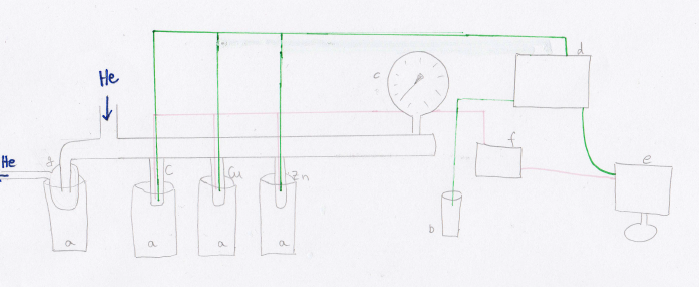
\includegraphics[scale=0.9]{VersuchsaufbauZeichnung.png} \end{center}
\caption{Versuchsaufbau.}
\end{figure}

a) Dewergefäß\\
b) Vergleichstemperaturbad ($T_{Soll}=$273,15 K)\\
c) Druckanzeige\\
d) Thermoelement\\
e) PC mit Labview\\
f) Heizsteuerung\\
g) Gasauffang\\
\subsection{Durchführung}
Die Messung erfolgte für jeden Stoff bei Zimmertemperatur, in einem Stickstoffbad und in einem Stickstoff/Ethanolbad und einem Heizstrom von 750~mA. Damit überall die gleiche Temperatur herrscht, wurde zunächst Helium durch die Apparatur geleitet und anschließend mittels Vakuum wieder abgezogen. Die Messung war in Vorlaufphase (60~s), Heizphase (20~s) und Endphase (200~s) unterteilt. Während der Heizphase wurde die auftretende Thermospannung inklusive Änderung (Fehler) notiert. Die Temperatur wurde mit einem Eisbad als Referenz mit dem Programm "Labview$"$ aufgezeichnet.\\



\section{Auswertung}


\subsection{Messergebnisse}
In der Tabelle 1 sind die Messergebnisse der Heizspannung sowie der Temperaturdifferenz dargestellt.
\begin{table}[h!]
\centering
\caption{Messergebnisse des Versuchs.}
\begin{tabular}{c|c|c|c|c|c|c}
T & Zimmertemperatur &Zimmertemperatur& $N_2$/EtOH& $N_2$/EtOH& $N_2$& $N_2$\\ 
& U[V]& $\Delta T$ [K]&U[V]& $\Delta T$ [K]&U[V]& $\Delta T$ [K]\\
\hline
Graphit & 4 & $3,22\pm0,01$ & 4,1 &$3,20\pm0,03$&4,6&$3,16\pm0,05$\\  
Kupfer & 1,2 & $3,72\pm0,02$ & 1 &$3,68\pm 0,01$&0,8&$3,61\pm0,03$\\ 
Zink & 1,4 & $3,61\pm 0,02$ & &$3,53\pm0,04$&0,8&$3,53\pm 0,09$ \\ 
\end{tabular} 
\end{table}
\FloatBarrier
\subsection{Bestimmung von $f$}

Die experimentell ermittelte molare Wärmekapazität bei konstantem Druck errechnet sich folgendermaßen:\\

\begin{equation}
c_{m,p} = \frac{UI\Delta t}{n\Delta T}
\end{equation}

Hierbei wurde ein Heizstrom $I$ von 750~mA und eine Heizzeit $\Delta t$ von 20~s eingestellt. Die Auswertungsergebnisse sind in der Tabelle 2 aufgelistet.
\begin{table}[h!]
\centering
\caption{Ergebnisse für $\text{c}_P^{\text{Exp.}}$.}
\begin{tabular}{c|c|c|c|c}
Probe& Spannungsabfall [V] & $\Delta$T [K]& Stoffmenge [mol] &  $\text{c}_P^{\text{Exp.}}$ [$\frac{\text{J}}{\text{mol}\cdot\text{K}}$]\\
\hline
Graphit & 3,22&4 &2,67 &4,52 \\
\hline
Zink & 3,72 & 1,2&0,900&51,7  \\
\hline
Kupfer & 3,61& 1,4& 0,692 &55,9\\
\end{tabular}
\end{table}
\FloatBarrier 

Der Korrekturfaktor \textit{f} ergibt sich aus dem Verhältnis von $\text{c}_P^{\text{Lit.}}$und $\text{c}_P^{\text{Exp.}}$. Die Korrekturfaktorenfür Graphit, Kupfer und Zink sind in Tabelle 3 dargestellt. 
\begin{equation}
f=\frac{\text{c}_P^{\text{Lit.}}}{\text{c}_P^{\text{Exp.}}}
\end{equation}
\begin{table}[h!]
\centering
\caption{Ergebnisse für $f$.}
\begin{tabular}{c|c|c}
Probe&$\text{c}_P^{\text{Lit.}}$ [$\frac{\text{J}}{\text{mol}\cdot\text{K}}$]&$f$\\
\hline
Graphit &8,517 &1,88 \\
\hline
Zink & 24,47&0,474  \\
\hline
Kupfer & 25,330&0,453\\
\end{tabular}
\end{table}
\FloatBarrier

Da die Messung des Spannungsabfalls fehlerbehaftet ist, wurde eine Gaussische Fehlerfortpflanzung aufgestellt um $\Delta\text{c}_P^{\text{Exp.}}$ und $\Delta f$ zu bestimmten:
\begin{align}
\Delta \text{c}_P^{\text{Exp.}}&=\sqrt{ \left(\frac{I\Delta t}{n\Delta T}\cdot \Delta U \right)^2}\\
\Delta \text{c}_P^{\text{Exp.}}(\text{Graphit bei ZT})&=\sqrt{ \left(\frac{750\cdot 10^{-3}\;\text{A} \cdot 20\;\text{s}}{2,67\;\text{mol}\cdot 4\;\text{K}}\cdot 0,01\;\text{V} \right)^2}\\
&=0,014 \;\frac{\text{J}}{\text{mol}\cdot\text{K}}
\end{align}
\begin{table}[h!]
\centering
\caption{Ergebnisse für $\Delta \text{c}_P^{\text{Exp.}}$.}
\begin{tabular}{c|c|c|c}
Probe&Temperaturbad&$\Delta U$ [V]&$\Delta \text{c}_P^{\text{Exp.}}$ [$\frac{\text{J}}{\text{mol}\cdot\text{K}}$]\\
\hline
Graphit& Zimmertemperatur&0,01&0,014\\
\hline
&Stickstoff&0,01&0,012\\
\hline
&Stickstoff/Ethanol&0,01&0,014\\
\hline
Zink &Zimmertemperatur&0,02& 0,309 \\
\hline
&Stickstoff&0,01&0,271\\
\hline
&Stickstoff/Ethanol&0,01&0,217\\
\hline
Kupfer &Zimmertemperatur&0,02& 0,278\\
\hline
&Stickstoff&0,01&0,208\\
\hline
&Stickstoff/Ethanol&0,01&0,167\\
\end{tabular}
\end{table}
\FloatBarrier
Die Ungenauigkeit des Korrekturfaktors $\Delta f$ ergibt sich ebenfalls aus der Fehlerfortpflanzung:
\begin{align}
\Delta f &= \sqrt{ \left(-\frac{\text{c}_P^{\text{Lit.}}}{(\text{c}_P^{\text{Exp.}})^2}\cdot \Delta \text{c}_P^{\text{Exp.}} \right)^2}\\
\Delta f (\text{Graphit})&= \sqrt{ \left(-\frac{8,517\;\frac{\text{J}}{\text{mol}\cdot\text{K}}}{(4,52\;\frac{\text{J}}{\text{mol}\cdot\text{K}})^2}\cdot 0,014\;\frac{\text{J}}{\text{mol}\cdot\text{K}}\right)^2}\\
&= 0,006\\
\Delta f (\text{Zink})&=0,003\\ 
\Delta f (\text{Kupfer})&=0,003\\
\end{align} 
Die Ergebenisse der experimentell bestimmten Wärmekapazitäten wurden mit den jeweiligen Korrekturfaktoren korrigiert und sind in der Tabelle 5 dargestellt.
\begin{table}[h!]
\centering
\caption{Ergebnisse.}
\begin{tabular}{c|c|c}
Probe&Temperaturbad&$\text{c}_P^{\text{Exp.}}$ [$\frac{\text{J}}{\text{mol}\cdot\text{K}}$]\\
\hline
Graphit& ZT&4,52 ± 0,014 \\
\hline
&$\text{N}_2$&7,27 ± 0,012 \\
\hline
&$\text{N}_2$/EtOH&8,26 ± 0,014 \\
\hline
Zink &ZT& 51,7 ± 0,309\\
\hline
&$\text{N}_2$& 35,6 ± 0,271\\
\hline
&$\text{N}_2$/EtOH& 29,0 ± 0,217\\
\hline
Kupfer &ZT&55,9 ± 0,278\\
\hline
&$\text{N}_2$&43,3 ± 0,208\\
\hline
&$\text{N}_2$/EtOH& 34,7 ± 0,167\\
\end{tabular}
\end{table}
\FloatBarrier
Die berechneten $\text{c}_P^{\text{Exp.}}$-Werte wurden gegen die Temperatur aufgetragen. Abbildung 3,4 und 5 zeigen den Kurvenverlauf für Grapgit, Kupfer und Zink.
\begin{figure} [h!]
\begin{center}
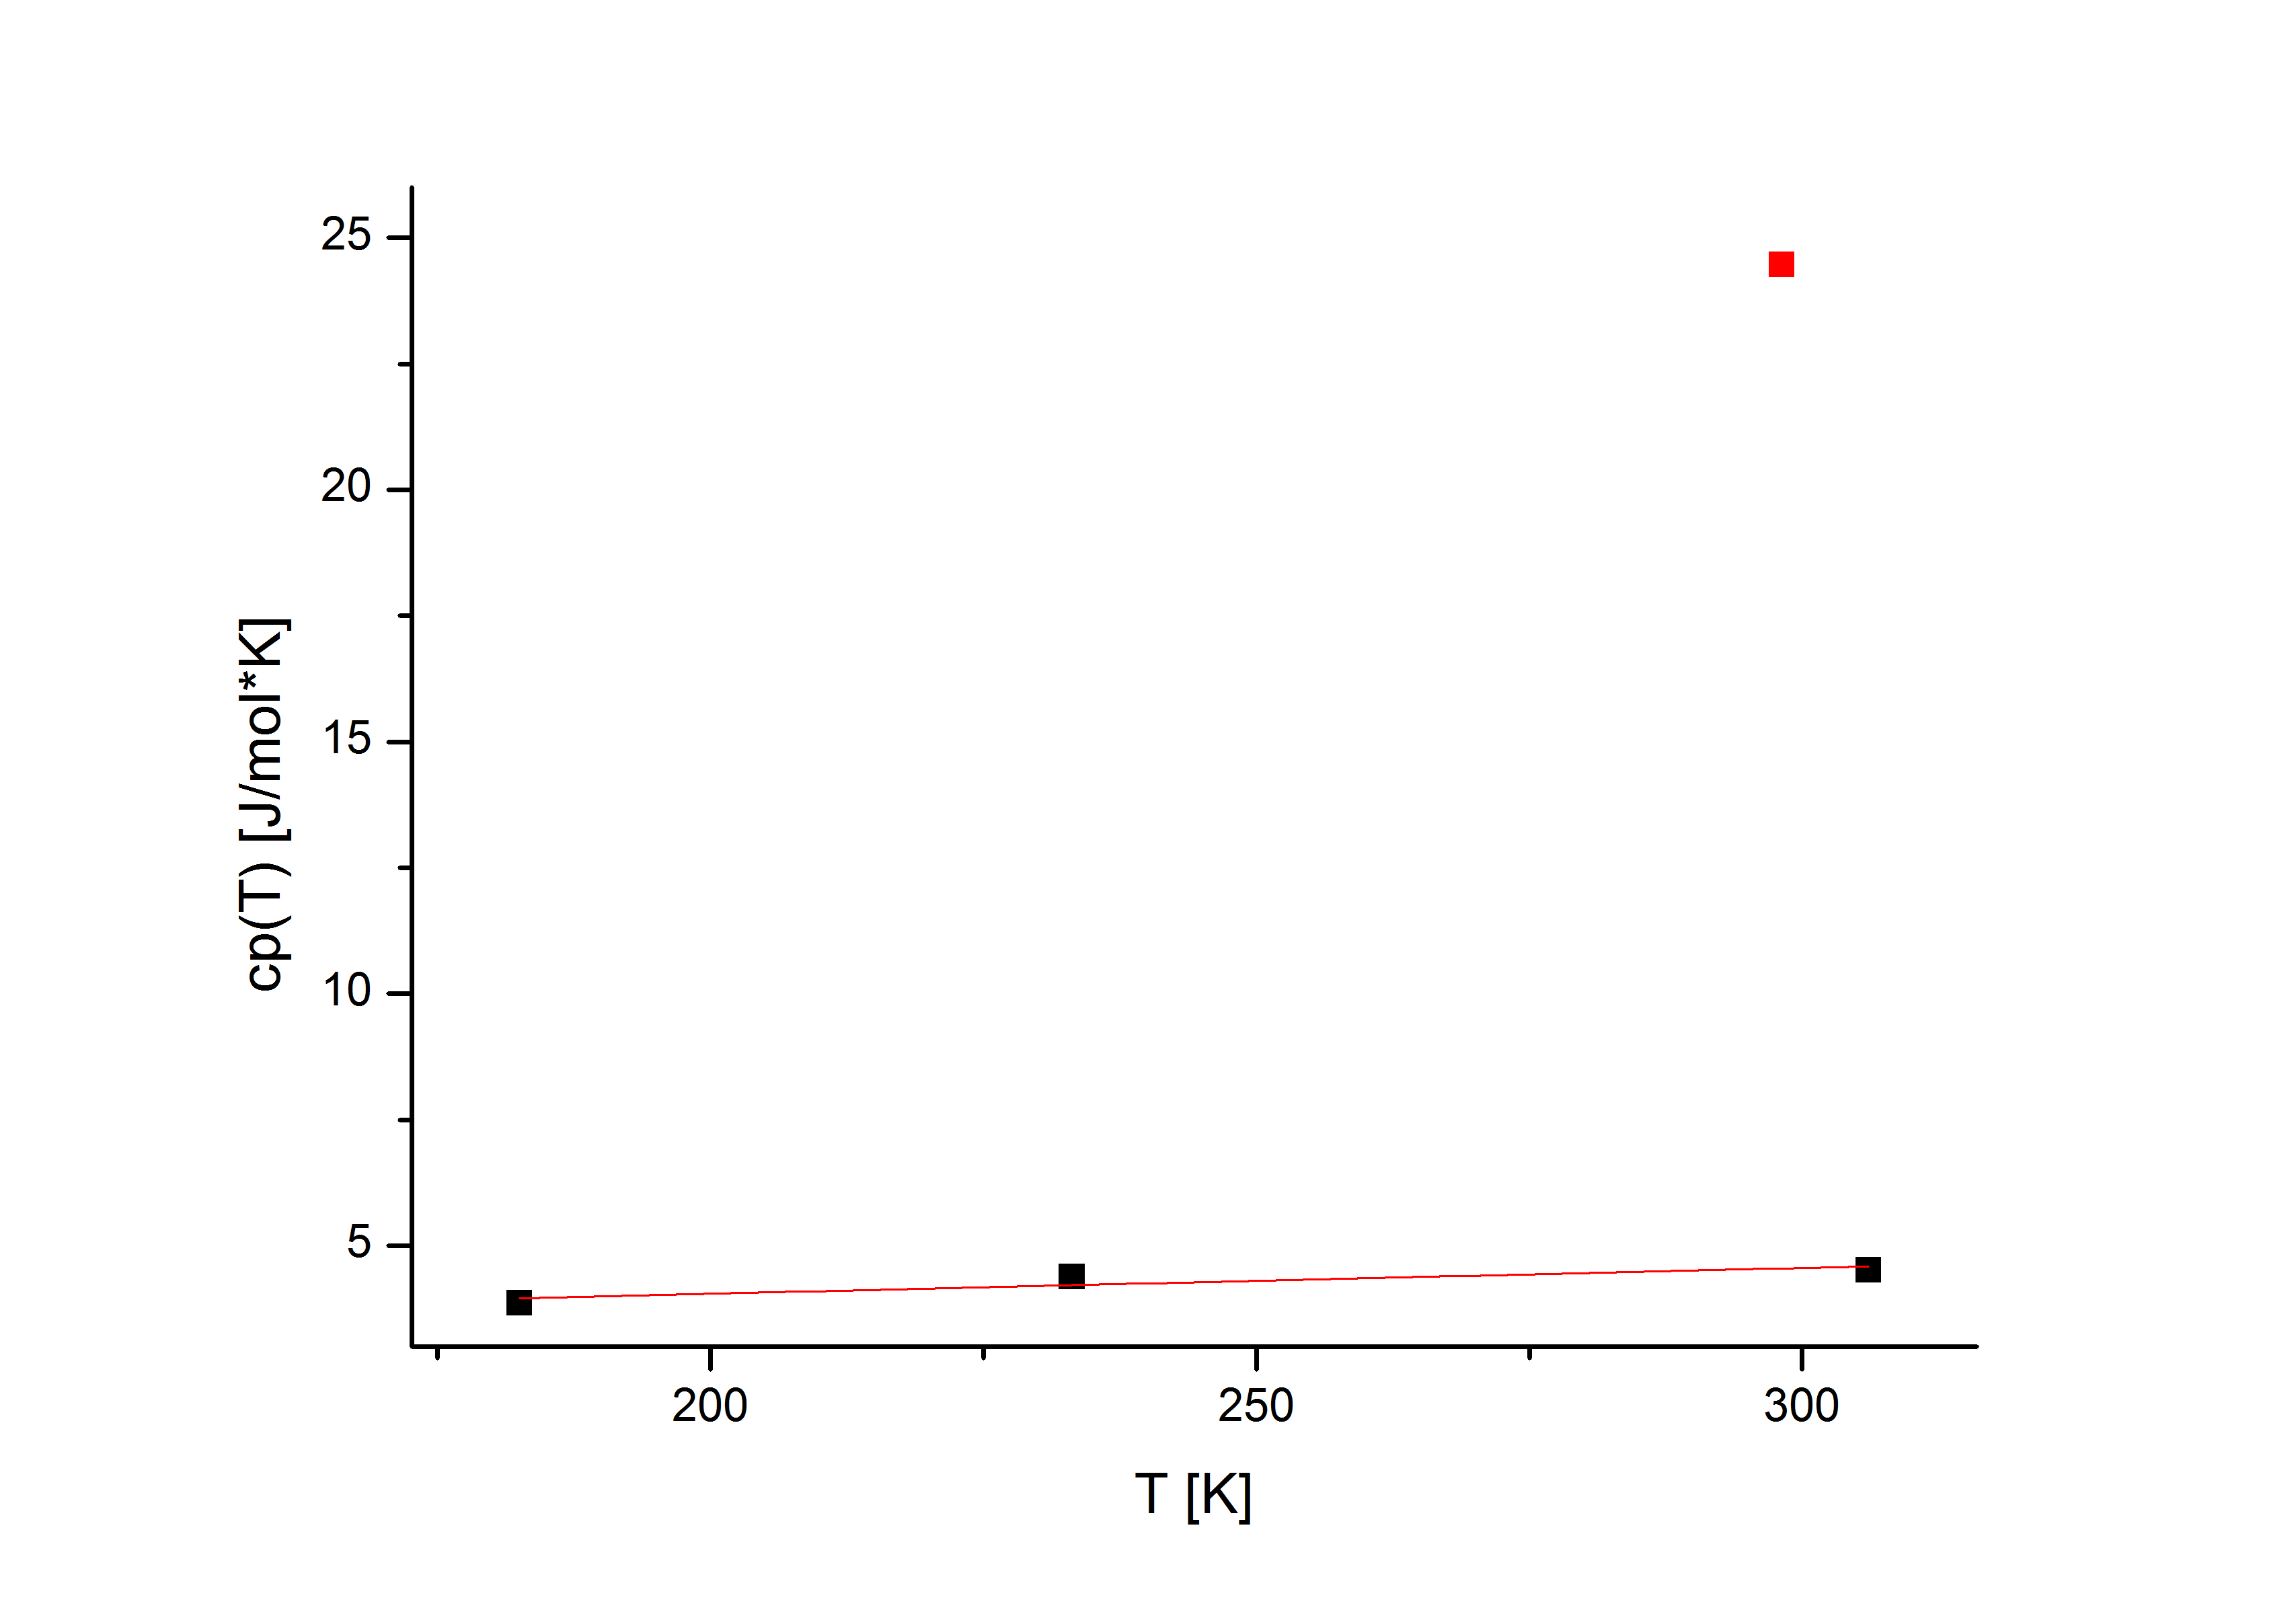
\includegraphics[scale=0.5]{cp(T)GraphitNeu.png} \end{center}
\caption{$c_p(T)$ Graphit, Literaturwert rot}
\end{figure} 
\FloatBarrier

\begin{figure} [h!]
\begin{center}
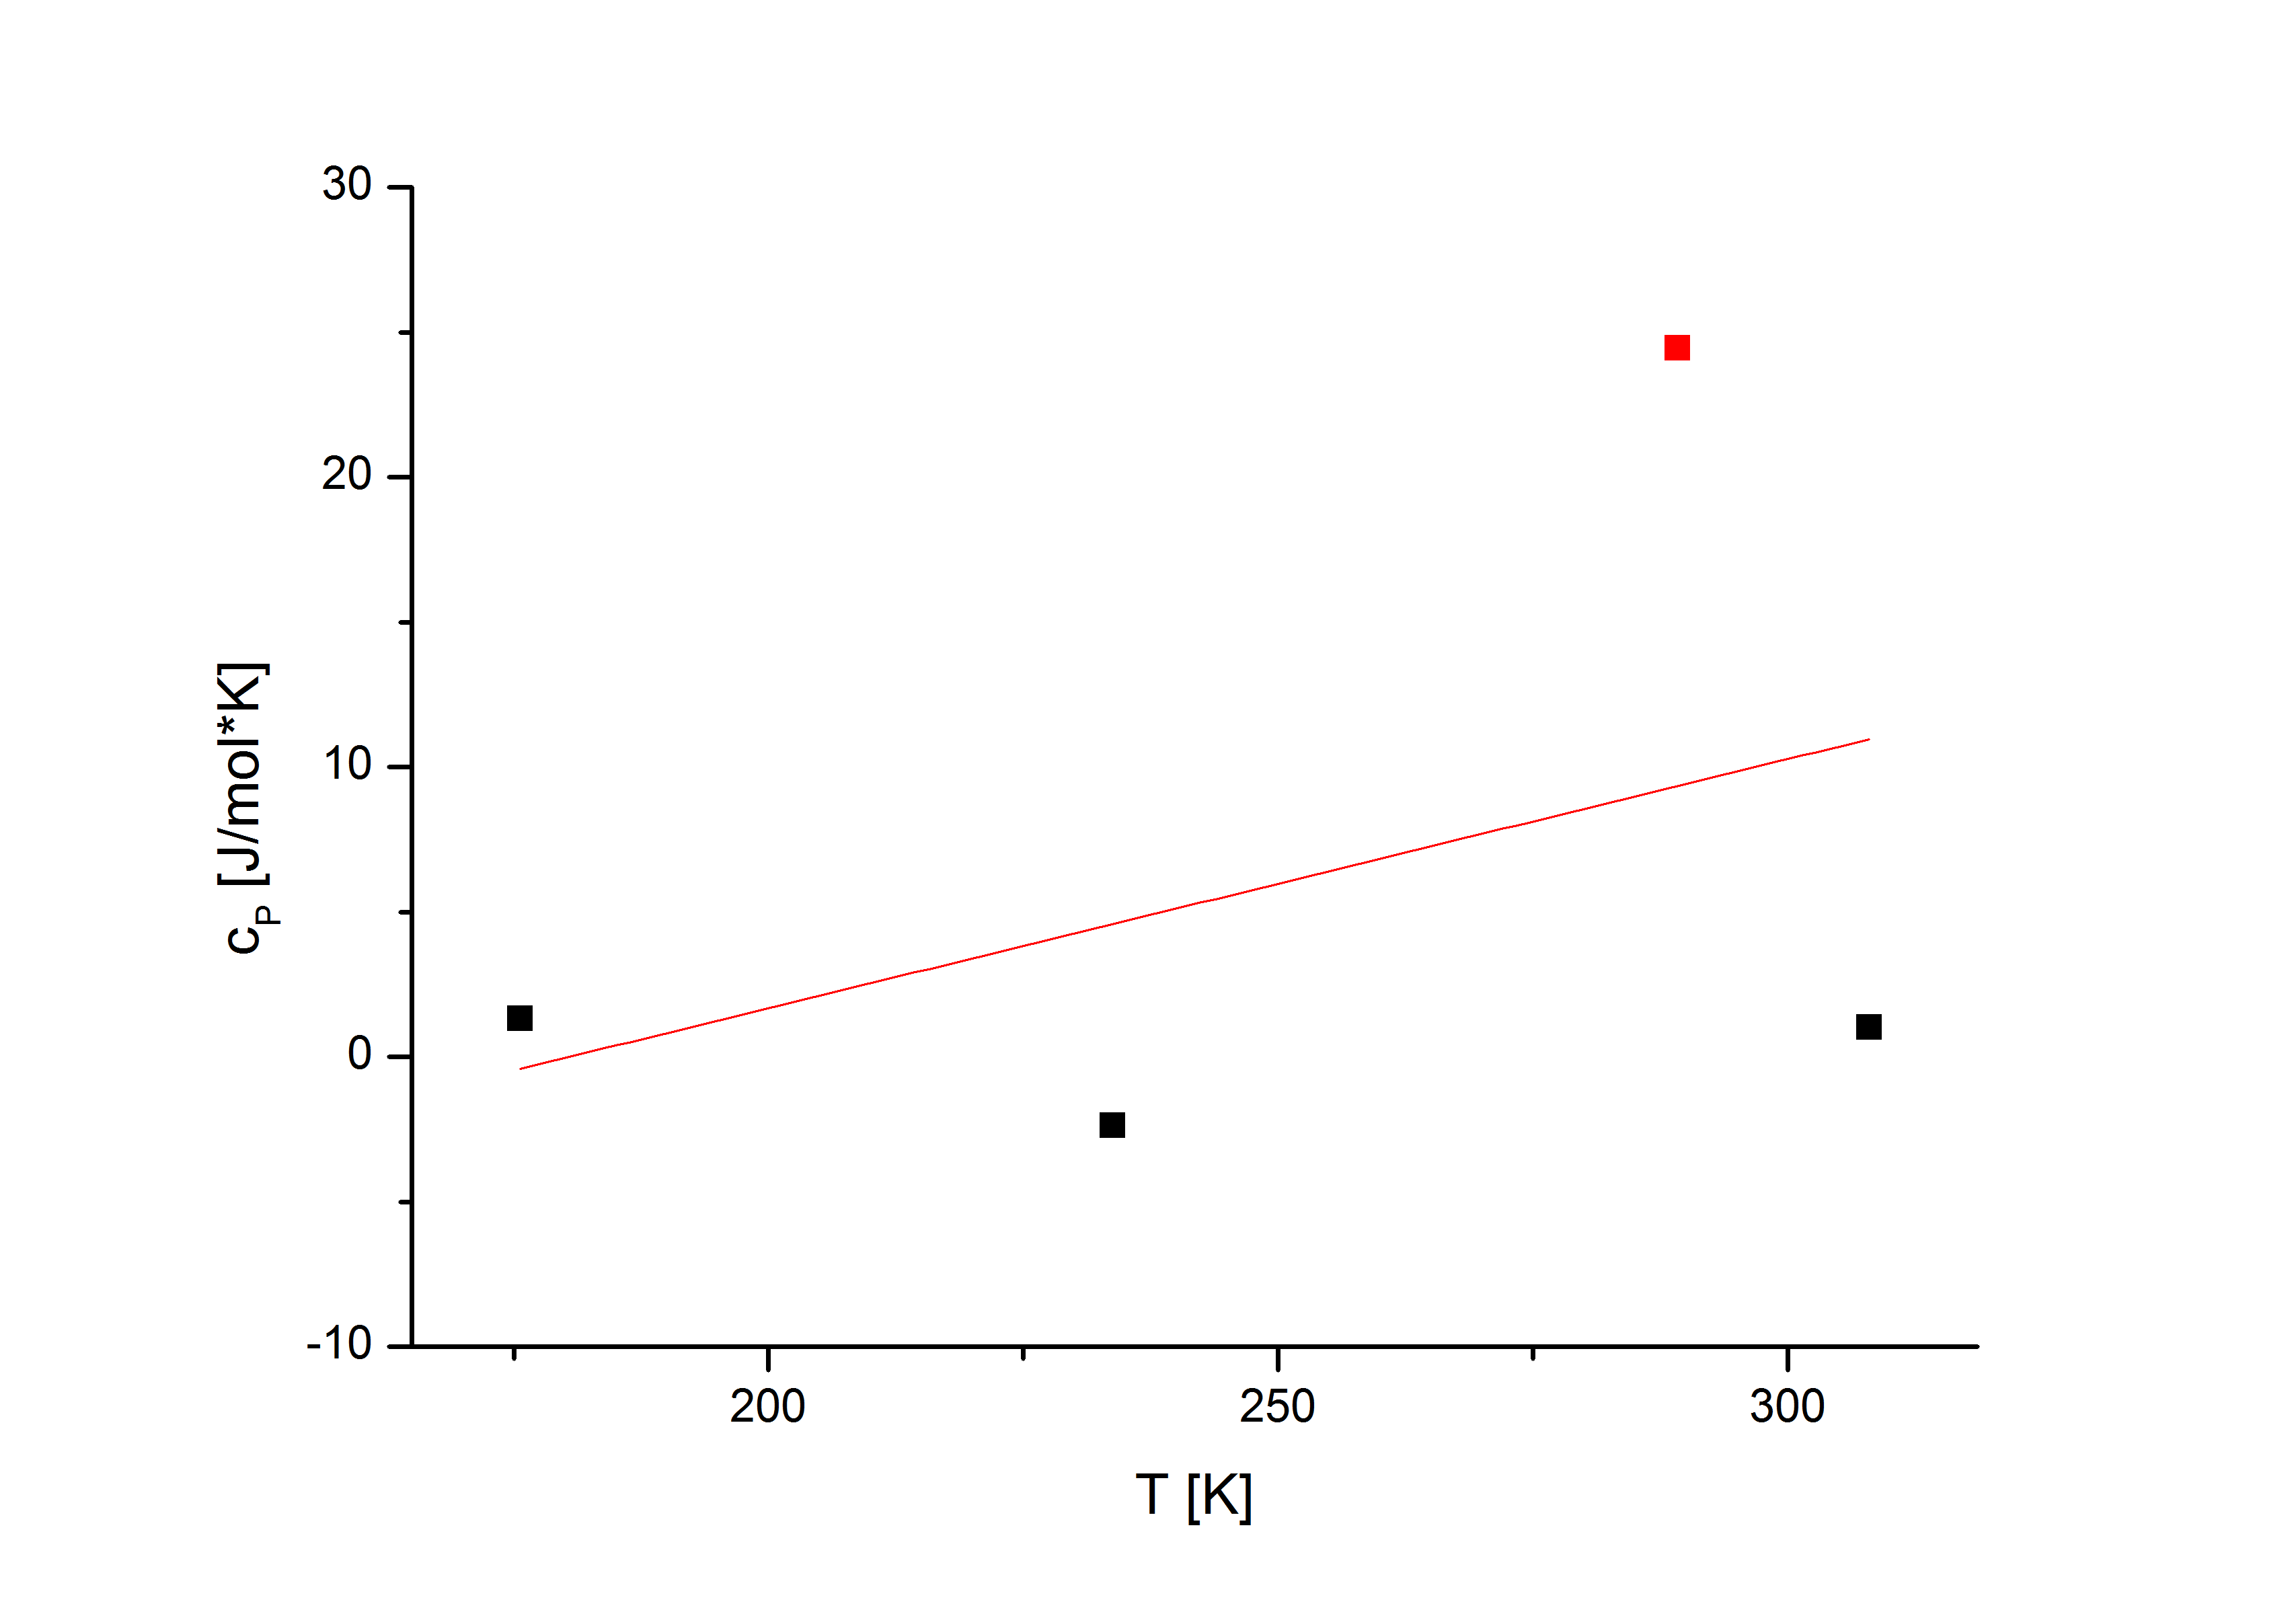
\includegraphics[scale=0.5]{cp(T)KupferNeu.png} \end{center}
\caption{$c_p(T)$ Kupfer, Literaturwert rot}
\end{figure} 
\FloatBarrier  

\begin{figure} [h!]
\begin{center}
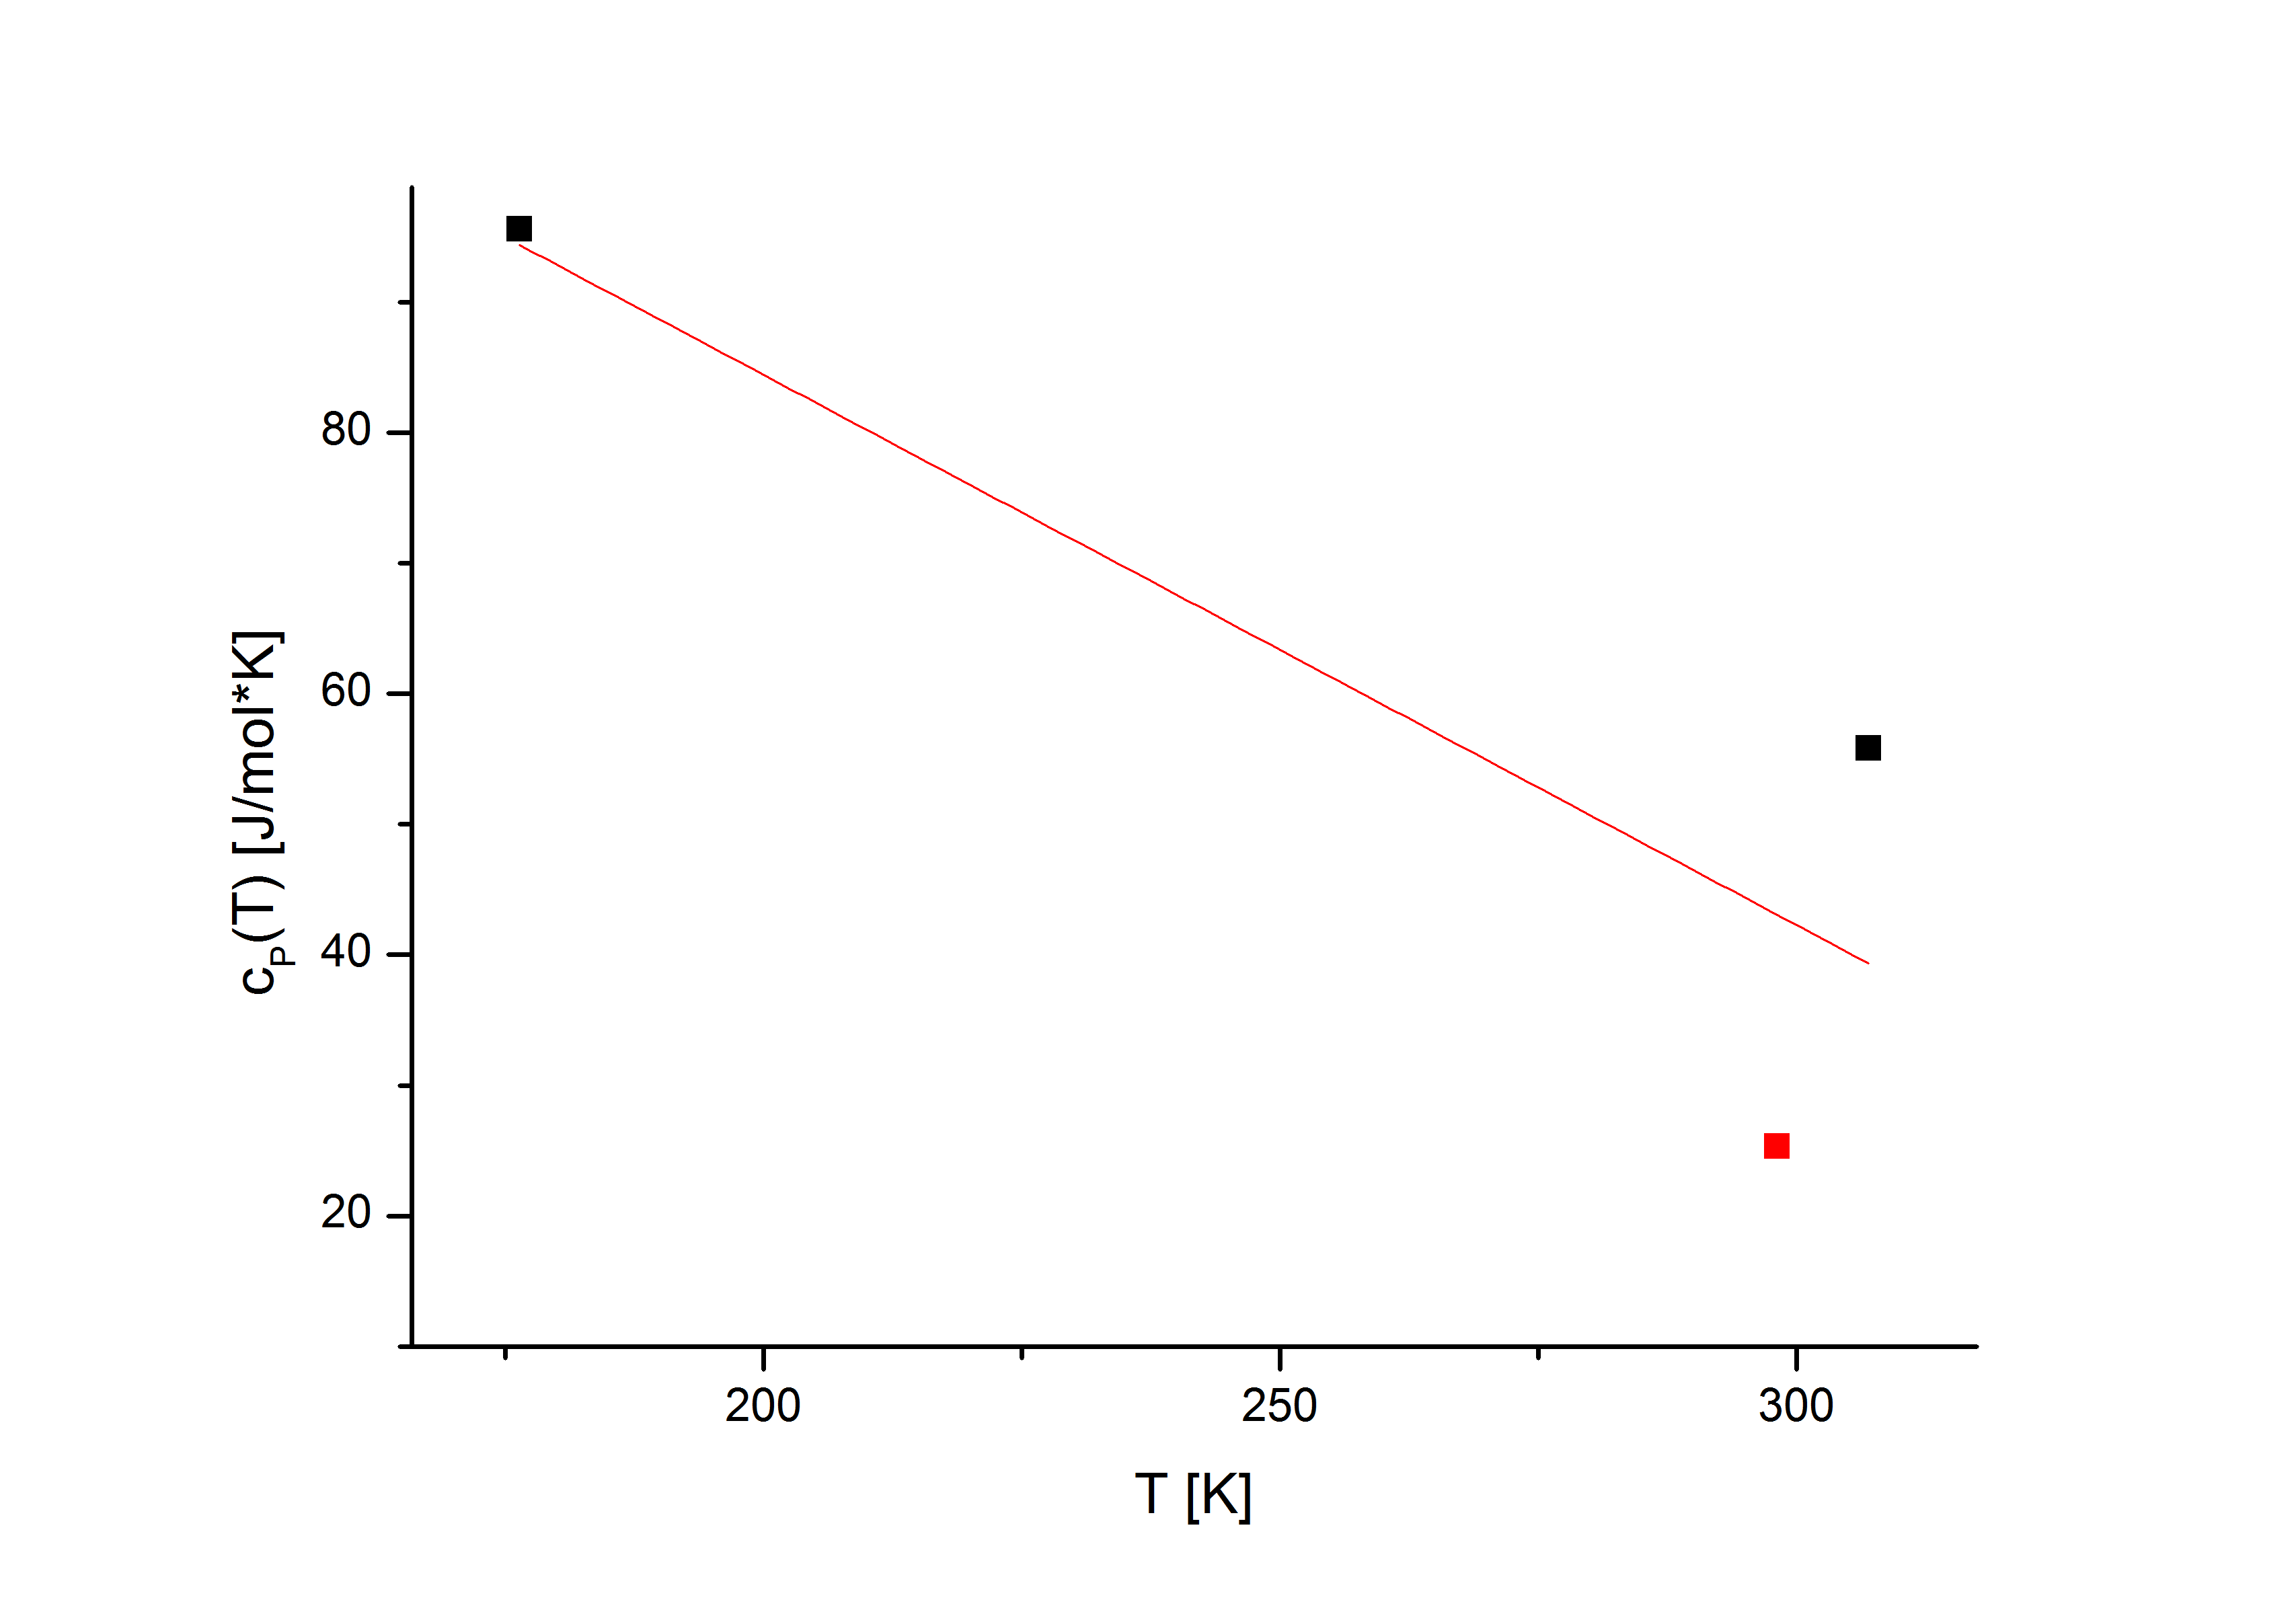
\includegraphics[scale=0.5]{Zinkcp(T)Neu.png} \end{center}
\caption{$c_p(T)$ Zink, Literaturwert rot}
\end{figure}    
\FloatBarrier 

      
Bei Zink und Kupfer wurde der Literaturwert in die lineare Interpolation mit einbezogen; die Abweichung vom Literaturwert bei Graphit war deutlich stärker als die Abweichung der Werte untereinander, sodass hier nur durch die Messwerte interpoliert wurde. Die Steigung und Ordinatenschnittpunkte finden sich in der nachfolgenden Tabelle.\\

\begin{equation}
c_p(T) = \left( m\cdot T  + n \cdot \mathrm{K} \right) \cdot \frac{\mathrm{J}}{\mathrm{mol}}
\end{equation}


\begin{table} [h] 
\centering
\caption{Werte zur linearen Interpolation}
\begin{tabular} {r | r|  r }
& Steigung $m$& Schnittpunkt mit Ordinate $n$\\
\hline
Graphit& 0,00512&3,0229\\
Cu&	0,0860	&-15,5\\
Zn&	-0,422	&169\\
\end{tabular}
\end{table}


\subsection{Berechnung von $c_{V}(T)$ nach Debye}
Die für verschiedene $\frac{T}{\Theta_{D}}$-Verhältnisse theoretischen Wärmekapazitäten der Stoffe können mittels Debye folgendermaßen berechnet werden:\\

\begin{equation}
c_{V}(T)= 3R \cdot \left(4 D(x) - \frac{3x}{e^x -1}\right)
\end{equation}

mit \\

\begin{equation}
D(x) = \frac{3}{x^3}\cdot \int_{0}^{x} \frac{t^3}{e^t -1} dt
\end{equation}

und $x= \frac{\Theta_D}{T}$.


%nachfolgende Tabelle mit den richtigen aktualisierten Werten
\begin{table} [h]
\centering
\caption{theoretische $c_V$-Werte nach Debye}
\begin{tabular} {r | r|  r | r}
&$\frac{T}{\Theta_D}=\frac{1}{x}$& D(x)&$c_V(T)[\mathrm{J}\cdot \mathrm{mol}^{-1} \cdot \mathrm{K}^{-1}]$\\
\hline
Graphit	&0,15&	0,0596	&5,31\\
	&0,2&	0,118	&9,20\\
	&0,25	&0,182&	12,5\\
	&0,3	&0,244	&15,2\\
	\hline			
Cu/Zn &	0,4	&0,354&	18,6\\
	&0,5&	0,441	&20,6\\
	&0,6	&0,510	&21,8\\
	&0,7&	0,564&22,6\\

\end{tabular}
\end{table}

\FloatBarrier

\subsection{Berechnung der zugehörigen $<\Theta_D>$-Werte }


Für Festkörper gilt: $c_V =c_p -R$, so kann die Gleichung auch auf die soben aus den Debye-Temperaturen ermittelten theoretischen $c_V(T)$- Werte angewendet werden. Somit können die zu den $c_V$- Werten zugehörigen Temperaturwerte ermittelt werden:\\

\begin{equation}
T= \frac{c_V(T) -n +R}{m}
\end{equation}

Zu den so errechneten Temperaturen werden die zugehörigen Debye-Temperaturen ermittelt nach:\\

\begin{equation}
T \cdot x = \Theta_D
\end{equation}

Letztendlich ergeben sich daraus folgende $\Theta_D$-Mittelwerte:\\


%aktualisierte Werte in dieser Tabelle 09.11.16
\begin{table} [h]\caption{$<\Theta_D>$ für jeweiliges Material}
\begin{tabular} {r | r|  r |r |r}
& $c_V$ [J/mol K] & T	[K] &$\Theta_D$ [$10^2\cdot$K]	&$<\Theta_D>$ [K]\\
\hline
Graphit &5,31	&2071	&138&	138$\cdot10^2$\\
        &9,20	&28,3&	141\\	
        &12,5&	34,8&	139\\	
        &15,1	&40,0	&133\\
\hline						
Cu &18,6 &	494 &	123$\cdot 10^1$ &	981\\
&20,6 &	517&	103 $\cdot 10^1$&\\
&21,8&	531 &	885& \\
&22,6 &	540 &	771&\\	
\hline			
Zn &18,6 &	336 &	841 &	630  \\
&20,6 &	332 &	663&  \\	
&21,8 &	329 &	548& \\	
&22,6 &	327& 	467& \\

\end{tabular}
\end{table}


\subsection{Auftragung $\frac{T}{\Theta_D}$}

%die Werte mussten nicht aktualisiert werden
\begin{table} [h]
\centering
\caption{Werte zur Auftragung von $c_V$ nach 2.3 gegen $\frac{T}{\Theta_D}$}
\begin{tabular} {r | r |r | r }
&$\Theta_{D,Lit}$ Literaturwert [K] &$c_V$ [J/mol K] aus 2.3& zugehöriges $\frac{T}{\Theta_{D,Lit}}$ \\
\hline
Graphit& 2500950\protect\footnote{Quelle: http://phycomp.technion.ac.il/~david/thesis/node3.html, aufgerufen am 06.11.16} &37,6&0,000122 \\
&&32,1& 0,0000730 \\
&&36,4& 0,0000932 \\
Cu&345\protect\footnote{Quelle: https://de.wikipedia.org/wiki/Debye-Temperatur, aufgerufen am 06.11.16} &430& 0,892 \\
&&625& 0,510\\
&&510& 0,677\\
Zn&308\protect\footnote{Quelle: http://www.spektrum.de/lexikon/physik/debye-temperatur/2809, aufgerufen am 06.11.16} &464& 0,997\\
&&795& 0,572\\
\end{tabular}
\end{table}

JULE AUFTRAGUNG MACHEN nd einfügen

\section{Diskussion}
\begin{table}[h!]
\centering
\caption{Ergebnisse.}
\begin{tabular}{c|c|c|c|c|c}
Probe&Temperaturbad&$\text{c}_P^{\text{Exp.}}$ [$\frac{\text{J}}{\text{mol}\cdot\text{K}}$] & $f$ &$\text{c}_P^{\text{Th.}}$ [$\frac{\text{J}}{\text{mol}\cdot\text{K}}$] &$\text{c}_P^{\text{Lit.}}$ [$\frac{\text{J}}{\text{mol}\cdot\text{K}}$] \\
\hline
Graphit& ZT&4,52 ± 0,014 &1,88 ± 0,006& &8,517 \\
\hline
&$\text{N}_2$&7,27 ± 0,012& & \\
\hline
&$\text{N}_2$/EtOH&8,26 ± 0,014 & &\\
\hline
Zink &ZT& 51,7 ± 0,309&  0,450 ± 0,003& &24,47\\
\hline
&$\text{N}_2$& 35,6 ± 0,271&&\\
\hline
&$\text{N}_2$/EtOH& 29,0 ± 0,217&&\\
\hline
Kupfer &ZT&55,9 ± 0,278& 0,474 ± 0,003& &25,330\\
\hline
&$\text{N}_2$&43,3 ± 0,208&&\\
\hline
&$\text{N}_2$/EtOH& 34,7 ± 0,167&&\\
\end{tabular}
\end{table}
\FloatBarrier
Temperatur des Vergleichsbades nicht konstant
komische Werte für T (10K zu viel)
bei letzter Messung iwas schief gelaufen- konnte nicht ausgewertet werden


\newpage


\subsection{Literaturverzeichnis}
1\quad Eckhold, Götz: \emph{Praktikum I zur Physikalischen Chemie}, Institut für Physikalische Chemie, Uni Göttingen, \textbf{2014}.
\vspace{0,5 cm}

2 \quad Eckhold, Götz: \emph{Statistische Thermodynamik}, Institut für Physikalische Chemie, Uni Göttingen, \textbf{2012}.

\vspace{0,5cm}

3 \quad Eckhold, Götz: \emph{Chemisches Gleichgewicht}, Institut für Physikalische Chemie, Uni Göttingen, \textbf{2015}.\\

\end{document}


